\documentclass[preprint,12pt,authoryear]{elsarticle}

\usepackage{amsmath,amssymb}
\usepackage{graphicx}
\usepackage{booktabs}
\usepackage{multirow}
\usepackage{url}
\usepackage[colorlinks=true,linkcolor=blue,citecolor=blue,urlcolor=blue]{hyperref}
\usepackage{xcolor}
\usepackage{enumitem}
\usepackage{algorithm}
\usepackage{algpseudocode}
\usepackage[mathlines]{lineno}
\setlength{\emergencystretch}{3em}
\usepackage{tikz}
\usetikzlibrary{arrows.meta}
\usepackage{pifont}

\definecolor{intentC}{HTML}{0072B2}
\definecolor{narrativeC}{HTML}{D55E00}
\definecolor{acousticC}{HTML}{009E73}
\definecolor{uncertaintyC}{HTML}{CC79A7}
\definecolor{figGray}{HTML}{8A8A8A}
\definecolor{figBg}{HTML}{F6F7F9}
\definecolor{passGreen}{HTML}{1E8449}
\definecolor{failRed}{HTML}{C0392B}

% ============================================================================
% 00_glossary.tex — 术语与记号宏（全文统一，防一词多义）
% 配套 main.tex v6.4+；正文统一引用此处记号。
% ============================================================================

% --- 模型家族与任务 ---
\newcommand{\LALM}{large audio-language model}
\newcommand{\LALMs}{large audio-language models}

% --- 析因因子记号（对应 §3.2 表）---
\newcommand{\Et}{\ensuremath{E_t}}      % 叙事文本框架 narrative text framing
\newcommand{\Nfac}{\ensuremath{N}}      % 叙事结构 narrative structure
\newcommand{\Rfac}{\ensuremath{R}}      % 角色分配 role assignment
\newcommand{\Asfac}{\ensuremath{A_s}}   % 声学风格 acoustic style

% --- 核心缩写 ---
\newcommand{\PCSD}{PCSD}
\newcommand{\pcsd}{paired cross-modal safety divergence}
\newcommand{\MSRF}{MSRF}
\newcommand{\msrf}{Multi-Source Risk Fusion}
\newcommand{\ASR}{attack success rate}

% --- 统计记号 ---
\newcommand{\pp}{\ensuremath{\,\mathrm{pp}}}       % percentage points
\newcommand{\OR}{odds ratio}
\newcommand{\ROC}{ROC-AUC}
\newcommand{\CI}[2]{\ensuremath{[#1,\,#2]}}        % 置信区间 [lo, hi]
\newcommand{\DeltaPP}{\ensuremath{\Delta}}         % 百分点差


\journal{Knowledge-Based Systems}

\begin{document}

\begin{frontmatter}

\begin{highlights}
\item Factorial study decomposes framing into text, structure, role, and acoustic style.
\item Narrative structure raises attack success by 27.9~pp (OR 16.65).
\item Paired cross-modal safety divergence is model-dependent, not modality-intrinsic.
\item MSRF is a knowledge-driven fusion of four signals (225 params; ROC-AUC 0.9784).
\item Honest reporting: defense gate G2 fails; fixed thresholds do not transfer.
\end{highlights}

\title{Cross-Modal Safety Inconsistency in Large Audio-Language Models: Measurement, Mechanism, and Knowledge-Driven Multi-Source Fusion}

\author[aff1]{Yongjin Chen}
\author[aff1,cor1]{Songze Zhu}
\ead{20196846@ppsuc.edu.cn}
\cortext[cor1]{Corresponding author}
\affiliation[aff1]{organization={People's Public Security University of China},country={China}}

\begin{abstract}
Large audio-language models (LALMs) are deployed in safety-sensitive decision
contexts, yet the safety implications of \emph{adversarial framing} ---
repackaging a fixed request through narrative, role-play, or acoustic style ---
remain poorly understood. We treat this as a \emph{knowledge-system} problem
and propose a knowledge-driven methodology: a safe decision must fuse
heterogeneous knowledge sources --- request intent, narrative structure,
acoustic style, and scoring uncertainty --- that current detectors represent
inconsistently or not at all. In a controlled paired factorial experiment
($E_t \times N \times R \times A_s$, 24 cells; 16{,}200 response cells; three
LALMs; two languages), narrative structure ($N$) raises attack success by
27.9 percentage points (95\% CI [25.0, 30.9]; odds ratio 16.65 [14.10,
19.67]). The effect is partially---not wholly---length-mediated and robust
across languages, models, and out-of-distribution anchors; the
agreement-conditioned dual-judge estimate (38.0~pp) is disclosed as
selection-inflated. We further
show paired cross-modal safety divergence (\PCSD) is model-dependent, so
audio vulnerability is not intrinsic to the modality. We then build \MSRF{}, a
knowledge-driven multi-source fusion framework that fuses these signal
families through calibrated out-of-fold scores in an auditable 225-parameter
layer. It reaches 0.9784 ROC-AUC on the deployment frame (0.9455 $\pm$ 0.030
cross-validation), outperforming billion-parameter guards, with boundaries
reported honestly (75.9\% benign false-positive rate; adaptive-attack decay).
Narrative structure exhibits a robust causal effect under controlled prompt
interventions; representing that effect as structured, multi-signal knowledge
is a more durable foundation for LALM safety than either modal shortcuts or
opaque detection.
\end{abstract}

\begin{keyword}
cross-modal consistency \sep knowledge-driven fusion \sep LALM safety \sep framing attack \sep causal attribution
\end{keyword}

\end{frontmatter}

\linenumbers

\section{Introduction}
\label{sec:intro}

Large audio-language models (LALMs) now power voice assistants, multimodal
customer service, and hands-free interaction, and are increasingly deployed in
safety-sensitive contexts. A growing body of work shows that such models can be
steered toward harmful output by \emph{adversarial framing}: keeping the
underlying request fixed while changing how it is packaged through narrative,
role-play, or acoustic style \citep{nyhm,pjbreak,stylebreak}. These attacks are
practical --- they require no gradient access, operate over the channel the
model was designed to consume, and are largely invisible to text-only
safeguards.

Yet the mechanisms behind framing attacks remain poorly understood. Prior work
treats ``delivery'' as a single coarse preset and compares whole attacks against
whole defenses. It does not ask \emph{which semantic component} --- the
emotional narrative text, the event-chain structure, the role assignment, or the
acoustic style --- drives attack success, nor whether these components interact.
Moreover, causal attribution has remained at the micro (internal) layer where it
is inaccessible to black-box practitioners, and existing audio safeguards are
rudimentary relative to their text counterparts.

\paragraph{Obstacles to component-level analysis.}
Three obstacles have blocked component-level analysis. First, framing components
are confounded with response length: narrative prompts elicit longer model
outputs, and length itself correlates with harmful content, so a naive
comparison cannot separate framing from verbosity
(Section~\ref{sec:length-mediation}). Second, safety judgment is itself
unreliable: single classifiers fail catastrophically on Chinese inputs (FNR
$\geq 0.96$ for three off-the-shelf scorers) and disagree with each other on
roughly one in six responses, so any measurement must rest on an audited
multi-scorer protocol (Section~\ref{sec:trust-chain}). It also means a
reliable safety decision cannot trust any single source and must fuse
heterogeneous, mutually non-overlapping signals
(Section~\ref{sec:msrf}). Third, \LALMs{} form a
heterogeneous family --- a finding that holds for one architecture may not hold
for another (Section~\ref{sec:crossmodal}).

\paragraph{Connection to Knowledge-Based Systems.}
We cast the problem as a \emph{knowledge-system} problem rather than only a
safety one. The four signals our study manipulates or measures --- request
intent, narrative structure, acoustic style, and scoring uncertainty --- are
four heterogeneous knowledge sources about a single decision (is this
interaction harmful?). \MSRF{} is a knowledge-fusion method that represents
each source's evidence, calibrates it, and combines it under uncertainty into
an auditable score. The paired cross-modal divergence (\PCSD) quantifies a
\emph{cross-modal knowledge inconsistency} --- the same request elicits
different safety-relevant knowledge through text versus audio. This aligns the
work with the knowledge-systems tradition of heterogeneous knowledge fusion,
uncertainty reasoning, and decision support
\citep{guo2024survey,shao2024duallevel,xu2025promethee,zhao2025ensemble,shafer1976}
and with recent KBS contributions that treat safety as a knowledge-
representation and decision-support problem \citep{srd,realignment}.

\paragraph{Contributions.}
We report a controlled, paired factorial study that decomposes the four framing
components across text and audio channels, a response-level cross-modal
consistency metric, and a signal-level fusion framework --- treating attack
mechanisms as structured, auditable, multi-signal knowledge rather than opaque
activations, an orientation shared with knowledge-based, decision-support
systems \citep{srd,realignment}. Concretely:

\begin{enumerate}[label=(\roman*)]
  \item \textbf{A knowledge-driven multi-source fusion framework.} We build
  \msrf{} (\MSRF), which represents four mutually non-overlapping signal
  families (harmful-intent semantics, narrative structure, acoustic prosody,
  and scoring uncertainty) as explicit knowledge sources and fuses them through
  out-of-fold calibration and a 225-parameter, auditable fusion layer. On the
  deployment frame it reaches 0.9784 \ROC{} (0.9455 $\pm$ 0.030 over five
  frames), outperforming ShieldGemma, WildGuard, and a reproduced GradSafe
  (ROC-AUC 0.198, 0.174, and 0.315, respectively) on the same test frame, while
  using roughly
  two--three orders of magnitude fewer parameters. We report its limits
  honestly: fixed-threshold detection does not transfer to benign inputs
  (75.9\% benign false-positive rate at the calibrated threshold), and adaptive
  attacks degrade detection (up to 20.0 pp). We therefore present \MSRF{} as a
  \emph{discriminative, in-distribution} framework for mechanism-aware risk
  scoring, not as a turnkey deployment defense.

  \item \textbf{Full-factorial causal attribution.} We manipulate \Et{}
  (narrative text framing), \Nfac{} (narrative structure / event-chain), \Rfac{}
  (role assignment), and \Asfac{} (acoustic style) in a 24-cell paired design
  over three \LALMs, two languages, and an out-of-distribution anchor set.
  Narrative structure is the dominant causal driver: on the full sample, attack
  success rises from 2.2\% to 30.1\% ($\Delta$27.9~\pp{} \CI{25.0}{30.9}; \OR{}
  16.65 \CI{14.10}{19.67}), with a consistent effect across languages (zh 29.3
  pp / en 26.6 pp), across models, and on the out-of-distribution AdvBench
  anchor ($\Delta$38.0 pp, dual-judge robustness caliber). A response-length
  covariate mediates a substantial share of the raw effect, supporting an
  \emph{elaboration-channel} account rather than a modality-intrinsic one. Role
  assignment has a \emph{negative} effect (\OR{} 0.53) --- a result we replicate
  and interpret rather than smooth over.

  \item \textbf{Response-level cross-modal consistency.} We quantify \pcsd{}
  (\PCSD) as a paired consistency score over the safety-relevant properties of
  the text and audio rendering of the same input, and show it is model-dependent
  (e.g., near-zero divergence for one architecture, strongly positive for two
  others) --- evidence that audio ``vulnerability'' is not intrinsic to the
  modality. We report it as an auxiliary diagnostic rather than a standalone
  contribution.
\end{enumerate}

We pre-registered two decision gates --- G1 (attribution established) and G2
(defense value); G1 passes, G2 does not, and we report both outcomes rather
than only the defense-positive one. The remainder of this paper presents the
protocol and factorial design (Section~\ref{sec:protocol}), the knowledge-driven
fusion framework and its formalization (Section~\ref{sec:msrf}), the attribution
results (Section~\ref{sec:attribution}), the cross-modal analysis
(Section~\ref{sec:crossmodal}), the fusion detection results and
their honest boundaries (Section~\ref{sec:fusion}), adaptive and degradation
robustness (Section~\ref{sec:robustness}), and discussion
(Section~\ref{sec:discussion}), followed by limitations
(Section~\ref{sec:limitations}) and conclusion
(Section~\ref{sec:conclusion}). Table~\ref{tab:novelty} positions this work
against the most related prior work across the four dimensions we contribute.

\begin{table}[t]
\centering
\caption{\textbf{Positioning against the most related prior work.} Compared
across the four dimensions of this paper's contribution. $\checkmark$ =
present; $\circ$ = partial (a single framing factor isolated without full
decomposition); $(\checkmark)$ = a benchmark-level aggregate rather than a
response-level measurement. All attributes follow the characterizations in
Section~\ref{sec:related}.}
\label{tab:novelty}
\footnotesize
{\setlength{\tabcolsep}{4pt}%
\begin{tabular}{lcccc}
\toprule
Work & Component-level & Cross-modal & Fusion-based & Honest boundary \\
     & attribution     & consistency  & defense      & reporting \\
\midrule
\citet{nyhm}            & -- & --       & -- & -- \\
\citet{pjbreak}         & $\circ$ & --   & -- & -- \\
\citet{stylebreak}      & -- & --       & -- & -- \\
\citet{omnisafetybench} & -- & $(\checkmark)$ & -- & -- \\
\citet{crossmodal-info} & -- & $\checkmark$ & -- & -- \\
\textbf{This work}      & $\checkmark$ & $\checkmark$ & $\checkmark$ & $\checkmark$ \\
\bottomrule
\end{tabular}}
\end{table}

\section{Related Work}
\label{sec:related}

\subsection{Framing and delivery attacks against LALMs}
Audio-side attacks on \LALMs have recently been shown to succeed via narrative
delivery \citep{nyhm} and prosody \citep{pjbreak}, and style-aware audio
jailbreaks \citep{stylebreak} demonstrate that acoustic style alone can steer
output. Paralinguistic variation, such as speaker emotion, similarly induces
safety inconsistencies \citep{feng2026emotional}, and a recent taxonomy
organizes audio jailbreaks into semantic, acoustic, signal, and embedding
layers, with narrative framing as a semantic-layer threat
\citep{feng2026audiojailbreaks}. These works establish that framing is a real
attack surface, but treat delivery as an atomic preset; none decomposes the
semantic components or measures their causal contributions under control
\citep{pjbreak,nyhm,stylebreak,feng2026emotional,feng2026audiojailbreaks}.
Our design differs on exactly this axis:
where \citet{nyhm} and \citet{stylebreak} compare whole attacks against whole
defenses, we decompose the ``storytelling'' bundle into four orthogonal
components (text, structure, role, acoustic style) and attribute success to
each under a paired control. Where \citet{pjbreak} varies prosody in
isolation, our acoustic factor is only one of four, and we disclose that it
confounds speaker identity and gender rather than claiming it isolates prosody
(Section~\ref{sec:setup}). Text-side research has taxonomized such persuasion
strategies \citep{wei2024}; our factorial design is the component-level
complement that quantifies their causal contribution in the audio-language
setting. The increment over this line of work is the decomposition itself:
rather than proposing a new delivery variant, we provide a reusable,
controlled measurement of \emph{which} framing component carries the effect,
under a paired design that separates structure from text, role, and acoustic
style.

\subsection{Safety benchmarks and consistency measurement}
Benchmarks such as HarmBench \citep{harmbench}, Audio Jailbreak
\citep{audio-jailbreak}, and Omni-SafetyBench \citep{omnisafetybench} evaluate
whether models or guards are safe on static collections, and Omni-SafetyBench
further defines a benchmark-level cross-modal consistency score (CMSC).
Consistency at the benchmark level, however, aggregates outcomes and cannot
localize per-input divergence between the text and audio rendering of the
\emph{same} query --- precisely where deployment disagreements originate. We
therefore define \PCSD{} at the response level as a measurement, not a
benchmark, and operationalize the distinction in
Section~\ref{sec:crossmodal} \citep{omnisafetybench}. The increment is
response-level granularity: \PCSD{} scores the text and audio rendering of
the \emph{same} input per cell, which a benchmark-level aggregate cannot
localize, and it is reported as an auxiliary diagnostic signal rather than a
label.

\subsection{Jailbreak detection and defense}
Jailbreak behavior in aligned models has been traced to brittle safety-training
boundaries \citep{jailbroken}, and detection approaches span gradient analysis
\citep{gradsafe}, input-output safeguards
\citep{llamaguard,shieldgemma,wildguard}, cross-modality consistency checking
for multimodal LLMs \citep{crossmodal-info}, confidence- and codebook-based
detection \citep{chen2025,codebooks}, and audio authenticity verification
\citep{xie2024fakesound}. These detectors share a single-cue
design: consistency disagreement \citep{crossmodal-info} or first-token
confidence \citep{chen2025,codebooks} alone, with no explicit
packaging-structure signal. Our fusion framework instead combines four mutually
non-overlapping, interpretable signal families and, unlike prior work, is
evaluated on both in-distribution discrimination and honest deployment
boundaries (Section~\ref{sec:fusion-boundary}). On the defense side,
inference-time refusal steering for \LALMs{} has also been proposed
\citep{lin2026sarsteer}. Within the
\emph{Knowledge-Based Systems} scope,
jailbreak mitigation has been framed as a model-agnostic semantic problem
\citep{srd} and safety as a subspace-oriented model-fusion objective
\citep{realignment}; the journal's orientation toward knowledge representation
and interpretable, decision-support detection is our target
\citep{srd,realignment}. Relative to this literature, our contribution is
three-fold: (a) causal attribution of \emph{which} framing component matters (a
knowledge question, not a classifier question); (b) a fusion framework whose
branches are mutually non-overlapping, interpretable signal families rather than
opaque embeddings; and (c) an honest evaluation that separates in-distribution
discrimination from deployment-level threshold behavior, which most detector
papers do not report.

\subsection{Knowledge fusion and decision-support systems}
Within the knowledge-systems tradition, safety-relevant and operational
decisions are supported by fusing heterogeneous knowledge sources under an
explicit treatment of uncertainty: belief-theoretic uncertainty reasoning and
quantification \citep{guo2024survey}, evidential (Dempster--Shafer) fusion of
multimodal information for reliable decisions \citep{shao2024duallevel},
multi-criteria fusion over multi-source decision data \citep{xu2025promethee},
and ensemble decisions over multimodal decision-information systems under
uncertainty \citep{zhao2025ensemble}. These works share a methodology that
this paper adopts: represent each source's evidence explicitly, calibrate or
discount it, and combine it under uncertainty to support a decision --- the
same structure that \MSRF{} instantiates for LALM safety scoring with four
mutually non-overlapping signal families \citep{shafer1976}. Our increment
over this line is twofold: the knowledge sources are \emph{response-level
signals extracted under a pre-registered causal protocol} rather than generic
features, and the fused decision is evaluated both for in-distribution
discrimination and for its honest boundary behavior (fixed-threshold
transfer), which decision-fusion studies typically do not report.

\section{Protocol and Factorial Design}
\label{sec:protocol}

\begin{quote}
\small\raggedright
Full machine-readable protocol: \texttt{RESEARCH\_PROTOCOL.md} v6.5 and
\texttt{STAGE\_CONTRACTS.md}; this section is the paper-facing summary.
\end{quote}

\subsection{Research questions and gates}
\begin{description}
\item[RQ1 (attribution).] Which framing component(s) causally increase attack
success in \LALMs{}, and are effects robust across language, model, and
out-of-distribution inputs?
\item[RQ2 (cross-modal).] Do text and audio renderings of the same input
diverge in safety judgment, and is the divergence model-dependent?
\item[RQ3 (detection).] Can a structured, signal-level fusion framework
discriminate framed attacks in-distribution, and how does it behave under
adaptive attack and audio degradation?
\end{description}

We pre-registered two decision gates. \textbf{G1} (attribution established)
requires a consistent, $\geq$10~pp effect whose bootstrap CI excludes zero under
the dual-judge caliber with acceptable scoring dispute. \textbf{G2} (defense
value) requires a significant TPR gain, $\geq$3 contributing branches, and a
benign false-positive rate $\leq$5\%. As reported in
Sections~\ref{sec:results} and \ref{sec:discussion}, G1 passes and
\textbf{G2 does not pass}; the paper therefore presents the attribution and
mechanism results as primary and the fusion framework as an application-level
validation with explicit boundary conditions.

\subsection{Factors and manipulation}
A paired factorial design \citep{fisher1935} varies four framing components
while holding the harmful request fixed:

\begin{table}[t]
\centering
\small
\caption{\textbf{The four framing factors.} Varied in the paired factorial
design (\S\ref{sec:setup}).}
\label{tab:factors}
\begin{tabular}{@{}l@{\hspace{2em}}p{0.30\textwidth}@{\hspace{2em}}p{0.28\textwidth}@{}}
\toprule
Factor & Definition & Levels \\
\midrule
\Et{} & Narrative text framing (emotional / narrative wording)
      & neutral vs.\ narrative \\
\Nfac{} & Narrative structure (event-chain packaging)
        & direct request vs.\ chained narrative \\
\Rfac{} & Role assignment (identity + task)
        & none vs.\ expert role \\
\Asfac{} & Acoustic style (TTS rendering)
         & neutral voice vs.\ styled voice \\
\bottomrule
\end{tabular}
\end{table}

Three templates instantiate each condition (9 templates total); a manipulation
check on response-level markers confirms each textual factor was delivered
(mean marker deltas 0.37--0.60, threshold 0.95 keep rate 1.0). We disclose that
the acoustic factor is implemented via TTS voices (a female neutral voice vs.\ a
male styled voice), so it confounds speaker identity and gender with prosody.
We do not claim \Asfac{} isolates prosody, and we verify no systematic length
difference across \Asfac{} variants (mean difference 1.18 chars, $p=0.24$).

\section{Experimental Setup}
\label{sec:setup}

\subsection{Models and scorers}
Three \LALMs{} constitute the model matrix: the two primary Gemma-4-family
models (E4B-it, audio+text; E2B-it, text) and Qwen2-Audio-7B as an architecture
control that is excluded from primary-effect inference. All Gemma-family models
run at BF16 with thinking disabled.

Safety judgment uses an audited multi-scorer protocol. Four scorers
(HarmBench-cls \citep{harmbench}, StrongREJECT \citep{strongreject}, and two
Gemma-family judges) are validated on an internal validation set (JailBench,
$n=602$)\footnote{JailBench is not a public benchmark; it is reported here for
reproducibility.}; the primary judge
(judge\_big) reaches 0.8555 accuracy. We define three calibers: \emph{primary}
(single best judge, full sample), \emph{dual-judge} (two judges agree, else
abstain), and \emph{majority} (four-vote). We use the \textbf{primary}
full-sample estimate for headline claims because it is the only caliber free of
a selection bias we disclose next. We use the \textbf{dual-judge} caliber for
cross-scorer robustness and for Chinese-language measurement, where single
scorers fail catastrophically (HarmBench FNR $=$ 1.0; StrongREJECT FNR $=$ 0.99)
while dual-judge reaches FNR 0.29 with 85.3\% accuracy (the third off-the-shelf
scorer, the Gemma-family judge, has FNR $=$ 0.96). Because the dual-judge
and majority calibers are defined only on rows where the two judges agree, and
agreement correlates with condition (in the confirmatory experiment,
storytelling rows are included at 57.9\% vs.\ 91.8\% for baseline), these
calibers systematically inflate the effect estimate ($\Delta$38.0 vs.\ 27.9~pp).
We report this agreement-conditioning selection bias in
Section~\ref{sec:results}. We further disclose that all internal scorers are
Gemma-family (three of the four majority votes; the four-vote majority
double-counts the E2B family leg), and that agreement with an independent
cross-family anchor (Qwen2.5-32B-Instruct-AWQ) is high (0.929 on the E4B side;
0.962 on the full E2B text set), which bounds the same-family risk.

\subsection{Statistical protocol}
Effects are reported as paired per-query cluster bootstraps \citep{efron1993}
($B=10{,}000$) with
95\% CIs, plus a Binomial Bayesian mixed-effects model \citep{bates2015} with
query random
intercepts and fixed model/template effects (the mixed-effect upgrade to full
random structure is not met --- fewer than three models and three templates ---
and is reported as such; the benchmark-level cross-frame fusion table uses
$B=2{,}000$). Paired per-query discordance is additionally tested with
McNemar's test \citep{mcnemar1947} on the baseline-safe/storytelling-harmful
versus
baseline-harmful/storytelling-safe cells; the asymmetry is strong across
languages and models (Chinese $\chi^2{=}34.6$, English $\chi^2{=}30.3$, E2B
$\chi^2{=}83.2$, E4B $\chi^2{=}91.1$; all $p<0.001$), and the same test is
applied after 1:1 nearest-neighbor length matching (caliper 0.2 SD). We
pre-registered TOST equivalence bounds ($\pm$5~pp) \citep{lakens2018},
O'Brien--Fleming sequential
alpha spending, and manipulation-check thresholds.
All generation is deterministic (byte-identical on re-run, 40/40), and decoding
robustness is verified under sampling ($\Delta$20.7~pp greedy vs.\
$\Delta$20.8~pp sampled, $n=48$).

% ============================================================================
% 05_fusion_framework.tex — MSRF 独立方法章（新 §5）
% 新版提示词 P1：将 MSRF 提升为独立方法章节，形式化 + 算法框 + 架构图。
% 全部数字与结构取自 stage_p2_msrf.py 与结果产物（见 REVISION_LOG R28）。
% ============================================================================
\section{A Knowledge-Driven Multi-Source Fusion Framework (MSRF)}
\label{sec:msrf}

Single-cue detectors are not trustworthy on framed inputs: off-the-shelf
harmfulness classifiers fail catastrophically on Chinese inputs (FNR
$\geq 0.96$; Section~\ref{sec:setup}) and the strongest open guards score
below chance on the framing distribution (Section~\ref{sec:fusion}). The
preceding analysis also establishes that the effect is carried by a specific,
identifiable component --- narrative structure --- not by generic ``attackness''
or modality. \MSRF{} is a knowledge-driven response to both facts: it
represents the evidence about a response as \emph{four mutually
non-overlapping knowledge sources}, calibrates each source's score, and fuses
them under an explicit uncertainty treatment into a single auditable score.
Figure~\ref{fig:msrf-framework} summarizes the architecture.

\begin{figure}[t]
\centering
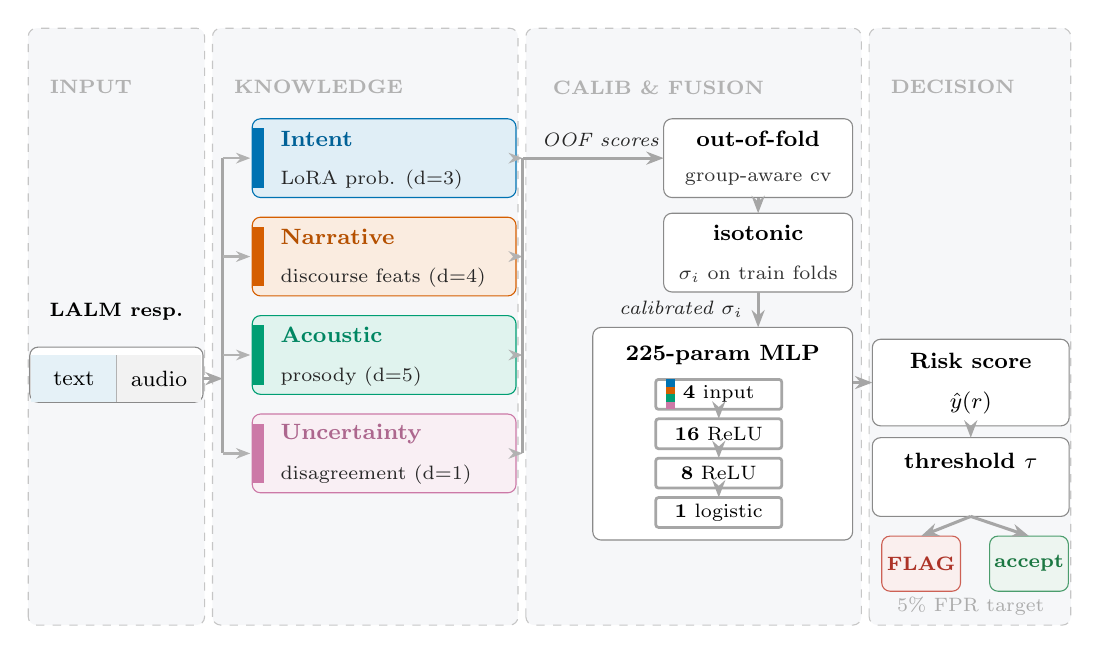
\begin{tikzpicture}[
  font=\footnotesize,
  bb/.style={rounded corners=3pt, draw=gray!45, dashed, fill=figBg},
  lbl/.style={font=\scriptsize\bfseries, text=gray!60},
  flw/.style={font=\scriptsize, text=gray!65},
  box/.style={rounded corners=2pt, draw=figGray, fill=white, inner sep=3pt},
  main/.style={-{Stealth[length=2.2mm]}, draw=gray!70, line width=1.1pt},
  aux/.style={-{Stealth[length=1.8mm]}, draw=gray!60, line width=0.8pt},
  bus/.style={draw=gray!70, line width=1.1pt},
]
% ---- swimlane bands (labels anchored top-left in reserved strip, inner margin >= 14pt) ----
\draw[bb] (0.08,0.12) rectangle (2.32,7.70);
\draw[bb] (2.42,0.12) rectangle (6.30,7.70);
\draw[bb] (6.40,0.12) rectangle (10.66,7.70);
\draw[bb] (10.76,0.12) rectangle (13.32,7.70);
\node[lbl, anchor=west] at (0.23,6.95) {INPUT};
\node[lbl, anchor=west] at (2.57,6.95) {KNOWLEDGE};
\node[lbl, anchor=west] at (6.62,6.95) {CALIB \& FUSION};
\node[lbl, anchor=west] at (10.91,6.95) {DECISION};

% ---- input: LALM response (title above box, >=6pt; text/audio dual channel) ----
\node[box, rounded corners=3pt, minimum width=2.2cm, minimum height=0.7cm] at (1.2,3.30) {};
\node[font=\scriptsize\bfseries] at (1.2,4.10) {LALM resp.};
\fill[intentC!10] (0.12,2.95) rectangle (1.20,3.55);
\fill[gray!10]    (1.20,2.95) rectangle (2.28,3.55);
\draw[gray!60]    (1.20,2.95) -- (1.20,3.55);
\node[font=\footnotesize] at (0.66,3.25) {text};
\node[font=\footnotesize] at (1.74,3.25) {audio};

% ---- knowledge sources (semantic colors + feature dims from Eqs.~1--4; d=3/4/5/1) ----
% Intent (blue, d=3)
\node[box, rounded corners=3pt, minimum width=3.35cm, minimum height=1.0cm,
      fill=intentC!12, draw=intentC] at (4.6,6.05) {};
\fill[intentC] (2.94,5.67) rectangle ++(0.14,0.76);
\node[right, font=\footnotesize\bfseries, text=intentC!85!black] at (3.16,6.30) {Intent};
\node[right, font=\scriptsize, text=black!85] at (3.16,5.78) {LoRA prob. (d=3)};
% Narrative (orange, d=4)
\node[box, rounded corners=3pt, minimum width=3.35cm, minimum height=1.0cm,
      fill=narrativeC!12, draw=narrativeC] at (4.6,4.80) {};
\fill[narrativeC] (2.94,4.42) rectangle ++(0.14,0.76);
\node[right, font=\footnotesize\bfseries, text=narrativeC!85!black] at (3.16,5.05) {Narrative};
\node[right, font=\scriptsize, text=black!85] at (3.16,4.53) {discourse feats (d=4)};
% Acoustic (green, d=5)
\node[box, rounded corners=3pt, minimum width=3.35cm, minimum height=1.0cm,
      fill=acousticC!12, draw=acousticC] at (4.6,3.55) {};
\fill[acousticC] (2.94,3.17) rectangle ++(0.14,0.76);
\node[right, font=\footnotesize\bfseries, text=acousticC!85!black] at (3.16,3.80) {Acoustic};
\node[right, font=\scriptsize, text=black!85] at (3.16,3.28) {prosody (d=5)};
% Uncertainty (purple, d=1)
\node[box, rounded corners=3pt, minimum width=3.35cm, minimum height=1.0cm,
      fill=uncertaintyC!12, draw=uncertaintyC] at (4.6,2.30) {};
\fill[uncertaintyC] (2.94,1.92) rectangle ++(0.14,0.76);
\node[right, font=\footnotesize\bfseries, text=uncertaintyC!85!black] at (3.16,2.55) {Uncertainty};
\node[right, font=\scriptsize, text=black!85] at (3.16,2.03) {disagreement (d=1)};

% ---- fusion chain ----
\node[box, rounded corners=3pt, minimum width=2.4cm, minimum height=1.0cm] at (9.35,6.05) {};
\node[font=\footnotesize\bfseries] at (9.35,6.30) {out-of-fold};
\node[font=\scriptsize, text=black!80] at (9.35,5.78) {group-aware cv};
\node[box, rounded corners=3pt, minimum width=2.4cm, minimum height=1.0cm] at (9.35,4.85) {};
\node[font=\footnotesize\bfseries] at (9.35,5.10) {isotonic};
\node[font=\scriptsize, text=black!80] at (9.35,4.58) {$\sigma_i$ on train folds};
% fusion MLP (title as first in-box line; 4 stacked layer boxes 4->16->8->1)
\node[box, rounded corners=3pt, minimum width=3.3cm, minimum height=2.7cm] at (8.9,2.55) {};
\node[font=\footnotesize\bfseries] at (8.9,3.55) {225-param MLP};
% layer 1: input (4) — left edge carries the four source colours
\draw[rounded corners=1pt, fill=white, draw=gray!70, line width=1pt]
  (8.05,2.86) rectangle (9.65,3.24);
\fill[intentC]      (8.18,3.145) rectangle (8.30,3.24);
\fill[narrativeC]   (8.18,3.05)  rectangle (8.30,3.145);
\fill[acousticC]    (8.18,2.955) rectangle (8.30,3.05);
\fill[uncertaintyC] (8.18,2.86)  rectangle (8.30,2.955);
\node[font=\scriptsize] at (8.85,3.05) {\textbf{4} input};
% layer 2: hidden 16 (ReLU)
\draw[rounded corners=1pt, fill=white, draw=gray!70, line width=1pt]
  (8.05,2.36) rectangle (9.65,2.74);
\node[font=\scriptsize] at (8.85,2.55) {\textbf{16} ReLU};
% layer 3: hidden 8 (ReLU)
\draw[rounded corners=1pt, fill=white, draw=gray!70, line width=1pt]
  (8.05,1.86) rectangle (9.65,2.24);
\node[font=\scriptsize] at (8.85,2.05) {\textbf{8} ReLU};
% layer 4: output 1 (logistic)
\draw[rounded corners=1pt, fill=white, draw=gray!70, line width=1pt]
  (8.05,1.36) rectangle (9.65,1.74);
\node[font=\scriptsize] at (8.85,1.55) {\textbf{1} logistic};
% inter-layer arrows (main style, >= 1pt)
\draw[main] (8.85,2.86) -- (8.85,2.74);
\draw[main] (8.85,2.36) -- (8.85,2.24);
\draw[main] (8.85,1.86) -- (8.85,1.74);

% ---- decision ----
\node[box, rounded corners=3pt, minimum width=2.5cm, minimum height=1.1cm] at (12.05,3.20) {};
\node[font=\footnotesize\bfseries] at (12.05,3.47) {Risk score};
\node[font=\footnotesize] at (12.05,2.94) {$\hat{y}(r)$};
\node[box, rounded corners=3pt, minimum width=2.5cm, minimum height=1.0cm] at (12.05,2.00) {};
\node[font=\footnotesize\bfseries] at (12.05,2.20) {threshold $\tau$};
\node[box, rounded corners=3pt, minimum width=1.0cm, minimum height=0.7cm,
      fill=failRed!8, draw=failRed!80] at (11.42,0.90) {};
\node[font=\scriptsize\bfseries, text=failRed!90!black] at (11.42,0.90) {FLAG};
\node[box, rounded corners=3pt, minimum width=1.0cm, minimum height=0.7cm,
      fill=passGreen!8, draw=passGreen!80] at (12.79,0.90) {};
\node[font=\scriptsize\bfseries, text=passGreen!90!black] at (12.79,0.90) {accept};
\node[flw] at (12.05,0.36) {5\% FPR target};

% ---- data-flow labels ----
\node[font=\scriptsize\itshape, text=black!85, anchor=west] at (6.48,6.28) {OOF scores};
\node[font=\scriptsize\itshape, text=black!85, anchor=east] at (9.28,4.13) {calibrated $\sigma_i$};

% ---- arrows ----
% input -> sources (fan-out bus)
\draw[main] (2.30,3.25) -- (2.55,3.25);
\draw[bus] (2.55,3.25) -- (2.55,6.05);
\draw[bus] (2.55,3.25) -- (2.55,2.30);
\foreach \y in {6.05,4.80,3.55,2.30} \draw[aux] (2.55,\y) -- (2.90,\y);
% sources -> fusion (converge bus; OOF scores annotated)
\foreach \y in {6.05,4.80,3.55,2.30} \draw[aux] (6.25,\y) -- (6.36,\y);
\draw[bus] (6.36,2.30) -- (6.36,6.05);
\draw[main] (6.36,6.05) -- (8.15,6.05);
% fusion chain
\draw[main] (9.35,5.55) -- (9.35,5.35);
\draw[main] (9.35,4.35) -- (9.35,3.90);
% fusion -> decision
\draw[main] (10.55,3.20) -- (10.80,3.20);
\draw[main] (12.05,2.65) -- (12.05,2.50);
\draw[main] (12.05,1.50) -- (11.42,1.25);
\draw[main] (12.05,1.50) -- (12.79,1.25);
\end{tikzpicture}
\caption{\textbf{The MSRF knowledge-driven fusion framework.} Four mutually
non-overlapping knowledge sources --- harmful-intent semantics (LoRA
probability, d=3), narrative structure (discourse features, d=4), acoustic
prosody (d=5), and scoring uncertainty (judge disagreement, d=1) --- are
extracted from each response, scored out-of-fold under group-aware splits
(OOF scores), calibrated with isotonic regression ($\sigma_i$), and fused by a
225-parameter MLP ($4\to16\to8\to1$) into a discriminative risk score
$\hat{y}(r)$; the operating threshold $\tau$ targets a 5\% FPR operating point
on the deployment frame. The honest boundary behavior of the framework (G2) is
reported in Section~\ref{sec:fusion-boundary}.}
\label{fig:msrf-framework}
\end{figure}

\subsection{Signal families as heterogeneous knowledge sources}
Each signal family is a knowledge source $i \in \{\mathrm{int},
\mathrm{nar}, \mathrm{ac}, \mathrm{unc}\}$ that produces a score
$x_i(r) \in [0,1]$ for a response $r$ (its text or audio rendering of the
same query):
\begin{align}
  x_{\mathrm{int}}(r) &= g_{\mathrm{int}}\!\big(p_{\mathrm{int}}(r),\,
      p_{\mathrm{int}}(r)^2,\, \ln\!\big(1+\ell(r)\big)\big), \label{eq:intent}\\
  x_{\mathrm{nar}}(r) &= g_{\mathrm{nar}}\!\big(\ell(r),\, n_{\mathrm{sent}}(r),\,
      d_{\mathrm{nar}}(r),\, n_{\mathrm{story}}(r)\big), \label{eq:narrative}\\
  x_{\mathrm{ac}}(r) &= g_{\mathrm{ac}}\!\big(f_0(r),\, e(r),\, \delta(r),\,
      \mathrm{zcr}(r),\, r_{\mathrm{sp}}(r)\big), \label{eq:acoustic}\\
  x_{\mathrm{unc}}(r) &= 2\cdot\min\!\big(p_{\mathrm{unc}}(r),\, 1-p_{\mathrm{unc}}(r)\big). \label{eq:uncertainty}
\end{align}
The intent source $x_{\mathrm{int}}$ is a LoRA fine-tuned harmful-intent
classifier over the E2B base whose input features are the intent probability,
its square, and normalized response length (\eqref{eq:intent}); the narrative
source $x_{\mathrm{nar}}$ uses interpretable discourse-structure features ---
length, sentence count, narrative density, and story-word presence
(\eqref{eq:narrative}); the acoustic source $x_{\mathrm{ac}}$ uses prosodic
features (f0, energy, duration, zero-crossing rate, speech/pause ratios) with
mean-imputation-plus-mask when audio is missing (\eqref{eq:acoustic}); and
the uncertainty source $x_{\mathrm{unc}}$ encodes scoring disagreement across
the multi-scorer protocol as $2\cdot\min(p,\,1-p)$, maximal when the scorer
consensus is maximally uncertain (\eqref{eq:uncertainty}). The families are
designed to be non-overlapping: each covers a disjoint aspect of the response,
so the fusion cannot ``double count'' the same evidence through two branches.
We disclose two boundary conditions of the sources: the intent branch was
trained in-distribution (its training rows overlap the evaluation set by
design of the stacking protocol), and the acoustic branch has no measurable
signal at our sample window ($N=32$ attacks). We phrase the latter as
``not measured'', not ``ineffective''.

\subsection{Fusion rule and parameter budget}
Branch scores are calibrated with isotonic regression $\sigma_i$ fit on
training splits to render them comparable across families, then fused by a
two-hidden-layer MLP $\mathcal{F}$:
\begin{align}
  \hat{y}(r) &=
    \mathcal{F}\!\Big(\sigma_1\big(x_{\mathrm{int}}(r)\big),\,
    \sigma_2\big(x_{\mathrm{nar}}(r)\big),\,
    \sigma_3\big(x_{\mathrm{ac}}(r)\big),\,
    \sigma_4\big(x_{\mathrm{unc}}(r)\big)\Big), \label{eq:fusion}\\
  |\mathcal{F}| &= (4\cdot 16 + 16) + (16\cdot 8 + 8) + (8\cdot 1 + 1) = 225. \label{eq:params}
\end{align}
The fused layer is a $4 \rightarrow 16 \rightarrow 8 \rightarrow 1$ ReLU MLP
with 225 trainable parameters (\eqref{eq:params}); the operating threshold
$\tau$ targets 5\% FPR on the deployment frame. The parameter budget is a
deliberate design choice: with 225 parameters the entire decision function is
inspecting three numbers per source, so every contribution to the score can be
traced back to an interpretable branch. This is an auditability property that
multi-billion-parameter guards (ShieldGemma-9B, WildGuard, GradSafe) do not
offer, and one we exploit to localize the honest boundary of the framework in
Section~\ref{sec:fusion-boundary}. This is the knowledge-fusion position of
\citet{shafer1976} and recent evidential fusion work
\citep{guo2024survey,shao2024duallevel,xu2025promethee}: evidence is made
explicit and combined under uncertainty, rather than buried in a black box.

\begin{table}[t]
\centering
\small
\caption{\textbf{The 225-parameter fusion budget.} Layer-by-layer composition
of the fusion MLP $\mathcal{F}$ ($4\to16\to8\to1$). The four inputs are the
isotonic-calibrated branch scores $\sigma_1,\dots,\sigma_4$ (intent, narrative,
acoustic, uncertainty); hidden activations are ReLU and the output is a
logistic layer, matching the scikit-learn \texttt{MLPClassifier} used in the
protocol (\texttt{hidden\_layer\_sizes=(16,8)}, \texttt{activation="relu"}).}
\label{tab:params}
\begin{tabular}{@{}llll@{}}
\toprule
Layer & Shape & Composition & Parameters \\
\midrule
1 & $4\to16$ (ReLU) & $4\times16+16$ & 80 \\
2 & $16\to8$ (ReLU) & $16\times8+8$ & 136 \\
3 & $8\to1$ (logistic) & $8\times1+1$ & 9 \\
\midrule
\multicolumn{3}{r}{\emph{Total trainable}} & \textbf{225} \\
\bottomrule
\end{tabular}
\end{table}

\subsection{Evaluation protocol}
Branch scores are produced \emph{out-of-fold} so that no row contributes its
own label to the score the fusion layer sees. The split is a group-aware
GroupShuffleSplit whose group key is template family $\times$ attack family
(21 groups), so that an entire template$\times$attack group is held out
together and leakage across conditions is prevented. An outer 25\% test frame
never participates in hyperparameter selection, and an inner 20\% validation
split selects the MLP learning rate. The protocol is repeated over five
independent seeds, yielding five independent test frames with the deployment
frame reported as primary. The silver ground-truth label is an
agreement-based subset of the multi-scorer protocol (66.2\% coverage; mean
pairwise agreement 0.8122), used only to train and score the fused detector.

Algorithm~\ref{alg:msrf} summarizes training and inference.

\begin{algorithm}[t]
\caption{MSRF training and inference}
\label{alg:msrf}
\begin{algorithmic}[1]
\Require responses $R$ (text/audio renderings); silver labels $L\subset R$;
        groups $G$ (template family $\times$ attack family)
\Ensure calibrated fusion model $\mathcal{F}$; threshold $\tau$
\Procedure{Train}{$R, L, G$}
  \For{each family $i \in \{\mathrm{int},\mathrm{nar},\mathrm{ac},\mathrm{unc}\}$}
    \State extract features and compute branch score $x_i(r)$ for all $r\in R$
    \State recompute branch scores out-of-fold over group-aware splits of $G$
  \EndFor
  \State fit isotonic calibrators $\sigma_i$ on the training splits
  \State select MLP learning rate on the inner 20\% validation split
  \State fit $\mathcal{F}: \mathbb{R}^4\to[0,1]$ (4$\to$16$\to$8$\to$1) on calibrated branch scores
  \State set $\tau$ to target 5\% FPR on the deployment-frame validation set
  \State \Return $\mathcal{F},\,\{\sigma_i\},\,\tau$
\EndProcedure
\Procedure{Infer}{$r$}
  \State compute $\{x_i(r)\}$; \Return $\mathcal{F}\big(\sigma_1(x_1),\dots,\sigma_4(x_4)\big)$
\EndProcedure
\end{algorithmic}
\end{algorithm}

\section{Results}
\label{sec:results}

Per the pre-registered protocol (Section~\ref{sec:protocol}), this section
reports the confirmatory attribution test under the primary caliber first,
then exploratory decompositions and diagnostic analyses; primary conclusions
are anchored to the pre-registered main-effect hypotheses, and all other
comparisons are reported as exploratory.

\begin{figure}[t]
\centering
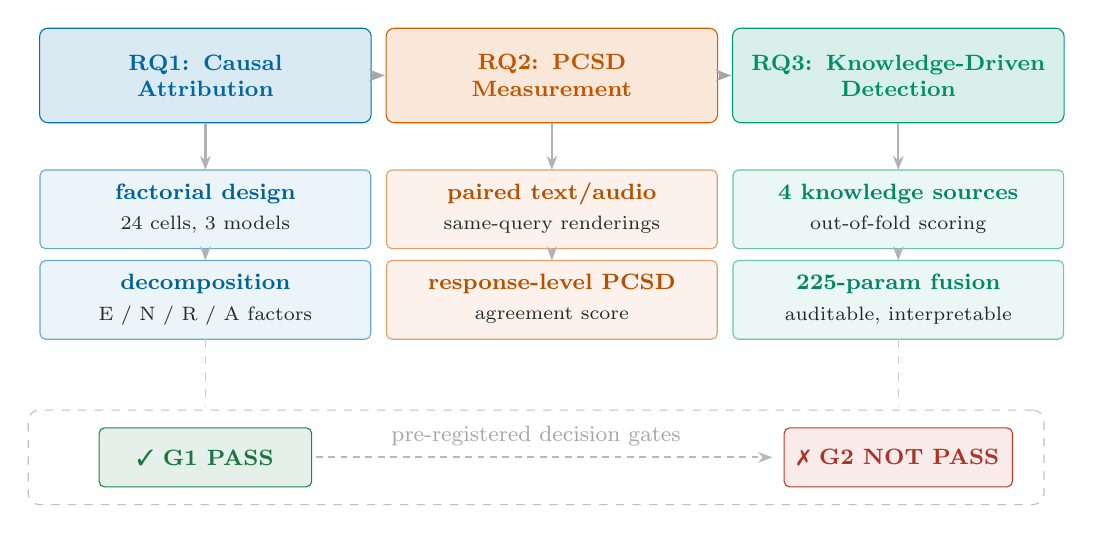
\begin{tikzpicture}[
  font=\footnotesize,
  stage/.style={rounded corners=3pt, minimum width=4.2cm, minimum height=1.2cm, inner sep=3pt},
  stnode/.style={rounded corners=2pt, minimum width=4.2cm, minimum height=1.0cm, inner sep=3pt},
  main/.style={-{Stealth[length=2mm]}, draw=gray!70, line width=1.1pt},
  aux/.style={-{Stealth[length=1.8mm]}, draw=gray!60, line width=0.8pt},
]
% ---- stage blocks (top layer, RQ1/RQ2/RQ3) ----
\node[stage, fill=intentC!15, draw=intentC, text width=4.0cm, align=center,
      font=\footnotesize\bfseries, text=intentC!90!black] at (2.5,6.0) {RQ1: Causal\\Attribution};
\node[stage, fill=narrativeC!15, draw=narrativeC, text width=4.0cm, align=center,
      font=\footnotesize\bfseries, text=narrativeC!90!black] at (6.9,6.0) {RQ2: PCSD\\Measurement};
\node[stage, fill=acousticC!15, draw=acousticC, text width=4.0cm, align=center,
      font=\footnotesize\bfseries, text=acousticC!90!black] at (11.3,6.0) {RQ3: Knowledge-Driven\\Detection};
\draw[main] (4.62,6.0) -- (4.78,6.0);
\draw[main] (9.02,6.0) -- (9.18,6.0);

% ---- step nodes (middle layer, same-hue shades) ----
% RQ1 (blue shades)
\node[stnode, fill=intentC!8, draw=intentC!60] at (2.5,4.30) {};
\node[font=\footnotesize\bfseries, text=intentC!85!black] at (2.5,4.50) {factorial design};
\node[font=\scriptsize, text=black!85] at (2.5,4.10) {24 cells, 3 models};
\node[stnode, fill=intentC!8, draw=intentC!60] at (2.5,3.15) {};
\node[font=\footnotesize\bfseries, text=intentC!85!black] at (2.5,3.35) {decomposition};
\node[font=\scriptsize, text=black!85] at (2.5,2.95) {E / N / R / A factors};
% RQ2 (orange shades)
\node[stnode, fill=narrativeC!8, draw=narrativeC!60] at (6.9,4.30) {};
\node[font=\footnotesize\bfseries, text=narrativeC!85!black] at (6.9,4.50) {paired text/audio};
\node[font=\scriptsize, text=black!85] at (6.9,4.10) {same-query renderings};
\node[stnode, fill=narrativeC!8, draw=narrativeC!60] at (6.9,3.15) {};
\node[font=\footnotesize\bfseries, text=narrativeC!85!black] at (6.9,3.35) {response-level PCSD};
\node[font=\scriptsize, text=black!85] at (6.9,2.95) {agreement score};
% RQ3 (green shades)
\node[stnode, fill=acousticC!8, draw=acousticC!60] at (11.3,4.30) {};
\node[font=\footnotesize\bfseries, text=acousticC!85!black] at (11.3,4.50) {4 knowledge sources};
\node[font=\scriptsize, text=black!85] at (11.3,4.10) {out-of-fold scoring};
\node[stnode, fill=acousticC!8, draw=acousticC!60] at (11.3,3.15) {};
\node[font=\footnotesize\bfseries, text=acousticC!85!black] at (11.3,3.35) {225-param fusion};
\node[font=\scriptsize, text=black!85] at (11.3,2.95) {auditable, interpretable};
% step arrows (within each stage)
\draw[aux] (2.5,5.40) -- (2.5,4.80);
\draw[aux] (2.5,3.80) -- (2.5,3.65);
\draw[aux] (6.9,5.40) -- (6.9,4.80);
\draw[aux] (6.9,3.80) -- (6.9,3.65);
\draw[aux] (11.3,5.40) -- (11.3,4.80);
\draw[aux] (11.3,3.80) -- (11.3,3.65);

% ---- gate band (bottom layer, G1/G2 timeline) ----
\node[rounded corners=4pt, draw=gray!50, dashed, fill=white,
      minimum width=12.9cm, minimum height=1.2cm] at (6.7,1.15) {};
\draw[aux, dash pattern=on 2.5pt off 2pt, draw=gray!55] (3.90,1.15) -- (9.70,1.15);
\node[font=\footnotesize, text=gray!70] at (6.7,1.42) {pre-registered decision gates};
\node[rounded corners=2pt, fill=passGreen!12, draw=passGreen,
      minimum width=2.7cm, minimum height=0.75cm] at (2.5,1.15) {};
\node[font=\footnotesize\bfseries, text=passGreen!90!black] at (2.5,1.15) {\ding{51} G1 PASS};
\node[rounded corners=2pt, fill=failRed!10, draw=failRed,
      minimum width=2.9cm, minimum height=0.75cm] at (11.3,1.15) {};
\node[font=\footnotesize\bfseries, text=failRed!90!black] at (11.3,1.15) {\ding{55} G2 NOT PASS};
% gate connectors
\draw[gray!40, line width=0.5pt, dashed] (2.5,2.65) -- (2.5,1.80);
\draw[gray!40, line width=0.5pt, dashed] (11.3,2.65) -- (11.3,1.80);
\end{tikzpicture}
\caption{\textbf{Study overview: from causal attribution through cross-modal
consistency to knowledge-driven detection.} RQ1 attributes attack success to
narrative structure ($\Delta$27.9~pp, OR 16.65); RQ2 quantifies response-level
paired cross-modal divergence (\PCSD{}) as model-dependent; RQ3 evaluates the
knowledge-driven fusion detector \MSRF{} (ROC-AUC 0.9784 on the deployment
frame). The pre-registered gates are reported honestly: G1 passes and G2 does
not (75.9\% benign false-positive rate at the calibrated threshold;
Section~\ref{sec:fusion-boundary}).}
\label{fig:overview}
\end{figure}

% ======================================================================
% RQ1 — Attribution
% ======================================================================
\subsection{Attribution (RQ1)}
\label{sec:attribution}

\subsubsection{Narrative structure is the dominant causal driver}
In the confirmatory full experiment (P1-FULL; 16,200 cells $=$ 600 queries
$\times$ 3 conditions $\times$ 3 templates $\times$ 3 models, where the 600
queries are 400 in-distribution --- 200 Chinese and 200 English --- plus 200
out-of-distribution AdvBench anchors; text modality),
storytelling framing raises attack success from \textbf{2.17\%} to
\textbf{30.08\%} under the primary (judge\_big) caliber on the full sample:
\textbf{$\Delta$27.9~pp} (95\% CI [25.04, 30.92]; mixed-model \textbf{OR 16.65}
[14.10, 19.67] with query random effects). The effect is robust in direction and
significance across all three calibers; the consistency calibers yield larger
magnitudes (dual-judge $\Delta$38.0~pp [33.98, 42.2]; majority $\Delta$36.8~pp)
because they are defined only on rows where the two judges agree, and agreement
correlates with condition (storytelling inclusion 57.9\% vs.\ baseline 91.8\%),
which systematically inflates these estimates. We disclose this
agreement-conditioning selection bias rather than smoothing it. The
unrestricted-creativity condition produces an intermediate effect ($\Delta$18.5~pp
on the dual robustness caliber), and the out-of-distribution AdvBench anchor
reproduces the storytelling effect under the same dual robustness caliber
($\Delta$38.0~pp; its odds ratio of 363 is inflated by the near-zero baseline and
is reported alongside the percentage-point effect).

\begin{figure}[t]
\centering

\includegraphics[width=0.82\textwidth]{figures/factorial_forest.pdf}
\caption{\textbf{Factorial forest plot.} Main and interaction effects of the
framing components on attack success under the primary caliber, estimated from
the pre-registered analysis; the zero line marks no effect, and the shaded band
marks the practically meaningful region ($\geq 10$~pp). Intervals are
cluster-bootstrap 95\% CIs ($B=10{,}000$); per-effect $n$ as labeled.}
\label{fig:factorial-forest}
\end{figure}

\subsubsection{Cross-lingual and cross-model robustness}
The effect is consistent across languages (Chinese $\Delta$29.3~pp, English
$\Delta$26.6~pp; interaction OR 1.41, $p<0.001$, i.e., a modestly stronger effect
in Chinese) and across the two primary models (E4B $\Delta$30.8~pp, E2B
$\Delta$25.1~pp) under the primary caliber; these per-language and per-model
estimates average to $\approx$27.9~pp, consistent with the pooled headline.
Under the dual-judge robustness caliber, the benchmark main table reproduces the
same ordering across the model$\times$language grid (range 29.9--40.2~pp), and
the architecture-control model Qwen2-Audio-7B reproduces the direction on text
(ASR 5.3\%$\rightarrow$38.8\%, $\Delta$33.5~pp) while being excluded from the
primary mixed model by design. Under our pre-registered cross-lingual
consistency rule the effect is judged robust in direction and magnitude.

\subsubsection{Benign control: framing amplifies existing intent}
On an independent benign-input control ($n=162$), storytelling framing produces
essentially no harmful output (0.0\% baseline, 3.2\% storytelling, 0.0\%
unrestricted; both flip directions zero). This supports an \emph{amplification}
account: framing does not conjure harmful behavior from benign inputs; it
amplifies existing harmful intent.

\subsubsection{The elaboration-channel hypothesis: length mediates a large share}
\label{sec:length-mediation}
The raw framing effect is confounded with response length: storytelling
responses average 937 characters versus 417 for baseline. In the pilot
factorial ($n=14{,}400$ cells), including a response-length covariate collapses
the \Nfac{} effect in the mixed-effects model (OR 1.49 without length vs.\ 1.03
with length). On the full data, however, within-length-band analyses retain a
substantive content effect: in the only band with real baseline samples
(200--799 chars) storytelling is not separable ($\Delta\approx{}+0.5$~pp), but in
the $\geq$800-char band --- where 96\% of storytelling responses fall --- the
storytelling effect is \textbf{+21.7~pp} (baseline 9.6\% vs.\ storytelling
31.3\%), and length-matching at $\geq$1012 chars still leaves \textbf{+17.5~pp};
the judge is not a ``long $\Rightarrow$ harmful'' shortcut, since baseline long
responses score only 9.6\% harmful. We therefore characterize the effect as
\emph{partially---not wholly---length-mediated} (elaboration-channel: framing
$\rightarrow$ longer elaboration $\rightarrow$ more harmful), with a real content
effect surviving within matched length bands. On the audio channel the three
estimators disagree in sign (single-slope OR 5.20; Mantel--Haenszel OR 0.60;
1:1 matched $-10.5$~pp, n.s.), and length-matched comparisons render
Qwen2-Audio's audio-channel effect negative ($-39.3$~pp, $p=0.003$). We report all
three estimators rather than a single favorable one, and we do \textbf{not}
claim that the audio modality is intrinsically more vulnerable.

\subsubsection{Component decomposition: N drives, R protects}
The factorial decomposition separates the components. Narrative structure
(\Nfac{}) carries the effect; narrative text framing (\Et{}) contributes a
smaller but significant effect; \textbf{role assignment (\Rfac{}) has a negative
effect} (OR 0.53, replicated across models) --- assigning the model an expert
identity makes harmful output \emph{less} likely in our protocol, a
counter-intuitive result we replicate and discuss in Section~\ref{sec:discussion}.
Interactions are modest: \Et{}$\times$\Rfac{} is significant in the pilot
(OR 2.54), and the \Nfac{} effect is stronger on audio than on text (pilot
dual-judge diff 7.26~pp; majority 9.84$\rightarrow$22.66 on audio vs.\
3.7$\rightarrow$8.38 on text). Family-level stratification shows the effect
generalizes across all five covered attack families (5/5 positive, 3/5
significant on dual-judge), with hate speech the most amplified
($\Delta\approx{}+17.6$~pp, roughly three times the overall effect;
\Nfac{}$\times$hate interaction significant in both models, $+13.5$~pp on E2B and
$+31.2$~pp on E4B); coverage excludes network attacks and benign requests. Of 84
pre-registered comparisons, 65 are significant, all surviving BH-FDR correction
\citep{benjamini1995} at $q=0.10$.

% ======================================================================
% RQ2 — Cross-modal consistency
% ======================================================================
\subsection{Cross-modal consistency (RQ2)}
\label{sec:crossmodal}

We quantify \textbf{paired cross-modal safety divergence} (\PCSD) through a
per-input \emph{agreement} score over the safety-relevant properties of a
model's response to the text rendering versus the audio rendering of the
\emph{same} query (length ratio and lexical overlap, combined 0.5/0.5; 0--1,
higher agreement $=$ less divergence). \PCSD{} is a response-level measurement,
distinct from benchmark-level consistency scores \citep{omnisafetybench}, and we
use the complementary audio-minus-text attack-success gap $\Delta$ as a
per-model divergence index.

Across the model matrix, \PCSD{} is \textbf{model-dependent}: agreement is
lowest for E4B (0.248) and highest for Qwen2-Audio (0.404), and the
audio-minus-text gap mirrors this ordering (E4B $+30.7$~pp, E2B $+44.6$~pp,
\textbf{Qwen2-Audio $-0.2$~pp}). Two implications follow. First, audio
``vulnerability'' is not intrinsic to the modality --- one architecture shows no
audio-text divergence at all. Input-side paralinguistic variation, such as
speaker emotion, likewise shifts \LALM{} safety outcomes
\citep{feng2026emotional}, reinforcing that inconsistency is a property of the
model--input interaction rather than of audio itself. Second, cross-modal
safety inconsistency is a
measurable, per-input phenomenon that a single modality-level metric would
obscure; this motivates treating cross-modal divergence as an auxiliary
diagnostic signal rather than a label.

\begin{figure}[t]
\centering
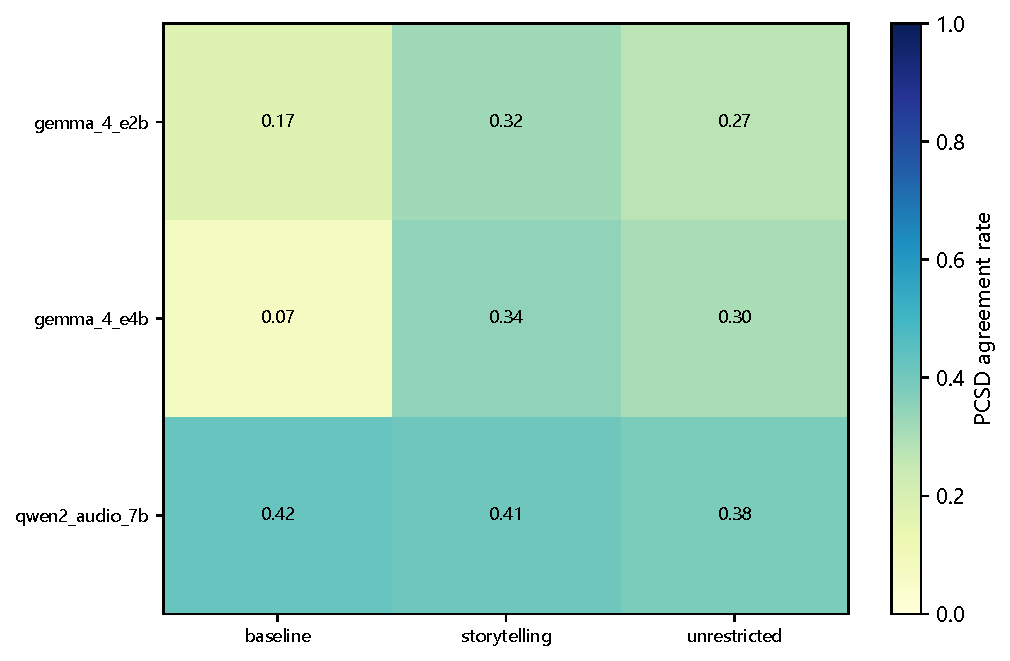
\includegraphics[width=0.72\textwidth]{figures/pcsd_heatmap.pdf}
\caption{\textbf{PCSD paired-divergence heatmap.} Response-level agreement and
divergence asymmetry between the text and audio rendering of the same query
under attack conditions, across models and framing conditions; darker cells
indicate higher agreement (less divergence). Per model $\times$ condition cell
$n$ as labeled.}
\label{fig:pcsd-heatmap}
\end{figure}

% ======================================================================
% RQ3 — Fusion framework
% ======================================================================
\subsection{A knowledge-driven fusion framework (RQ3)}
\label{sec:fusion}

\subsubsection{Design}
\MSRF{} is presented as a self-contained method in
Section~\ref{sec:msrf}: four mutually non-overlapping knowledge sources
(harmful-intent semantics, narrative structure, acoustic prosody, scoring
uncertainty), out-of-fold group-aware scoring, isotonic calibration, and a
225-parameter auditable fusion layer. We restate the headline protocol here
for continuity and evaluate the framework below.

\subsubsection{In-distribution discrimination}
On the deployment frame ($n=3{,}863$, 3.6\% positive), \MSRF{} reaches
\textbf{ROC-AUC 0.9784}, PR-AUC 0.6119, TPR@FPR5 0.8345, ECE 0.0299. Over five
independent group-split frames (protocol in Section~\ref{sec:msrf}; each frame
is that seed's group-aware test split, with the MLP learning rate selected on
an inner 20\% validation split so test rows never participate in selection),
mean ROC-AUC is \textbf{0.9455 $\pm$ 0.030} (min 0.8909, max 0.9784). The
weakest frame still outperforms the strongest open-source classifier by
$2.8\times$ (Table~\ref{tab:frames}).

\begin{table}[t]
\centering
\caption{\textbf{Cross-frame evaluation of the fused detector.} Five
independent group-aware GroupShuffleSplit test frames (group key $=$ template
family $\times$ attack family, 21 groups; outer 25\% test, inner 20\%
validation for learning-rate selection; Section~\ref{sec:msrf}). Frame 20260811
is the deployment frame used for all baseline comparisons.}
\label{tab:frames}
\small
\begin{tabular}{lrrrr}
\toprule
Seed & Test $n$ & ROC-AUC & PR-AUC & TPR@FPR5 \\
\midrule
20260811 (deployment) & 3{,}863 & \textbf{0.9784} & 0.6119 & 0.8345 \\
20260812 & 2{,}198 & 0.8909 & 0.6804 & 0.4608 \\
20260813 & 3{,}323 & 0.9447 & 0.4750 & 0.6071 \\
20260814 & 4{,}242 & 0.9667 & 0.7015 & 0.7891 \\
20260815 & 3{,}149 & 0.9470 & 0.5555 & 0.5539 \\
\midrule
Mean over 5 frames & -- & 0.9455 $\pm$ 0.030 & -- & -- \\
\bottomrule
\end{tabular}
\end{table}

\begin{figure}[t]
\centering

\includegraphics[width=0.78\textwidth]{figures/msrf_roc_pr.pdf}
\caption{\textbf{MSRF ROC/PR curves.} Detection performance of the real fused
detector on the deployment frame ($n=3{,}863$, 3.6\% positive). Solid curves are
the 5-seed mean with a 10--90 percentile envelope (mean ROC-AUC 0.9455 $\pm$
0.030; the deployment frame achieves 0.9784).}
\label{fig:msrf-roc-pr}
\end{figure}

Leave-one-branch-out ablation, evaluated
relative to the five-frame mean AUC (0.9455), shows intent and narrative carry
the signal (removing them drops AUC to 0.9136 and 0.9325, i.e., by 0.032 and
0.013) while the acoustic and uncertainty branches contribute marginally
(removal changes AUC by $\leq$0.001, to 0.9449 and 0.9448). Table
\ref{tab:ablation} reports the full ablation alongside each branch's
standalone score: the acoustic branch alone is chance-level (0.5, no signal
at our sample window), and the two best branches alone (intent 0.9325,
narrative 0.9136) each fall short of the fused detector, so the fusion
gain is not attributable to any single knowledge source.

\begin{table}[t]
\centering
\caption{\textbf{Leave-one-branch-out (LOO) ablation and single-branch
performance.} Evaluated relative to the five-frame mean AUC (0.9455). The
acoustic branch has no measurable signal at our sample window ($N=32$ attacks;
reported as ``not measured''), and the uncertainty branch has no standalone
score.}
\label{tab:ablation}
\small
\begin{tabular}{lccc}
\toprule
Branches & LOO ROC-AUC & $\Delta$ vs.\ full & Single-branch ROC-AUC \\
\midrule
Full (all four) & 0.9455 & -- & -- \\
$-$ intent & 0.9136 & $-0.032$ & 0.9325 $\pm$ 0.033 \\
$-$ narrative & 0.9325 & $-0.013$ & 0.9136 $\pm$ 0.048 \\
$-$ acoustic & 0.9449 & $-0.001$ & 0.5 $\pm$ 0.0 (no signal) \\
$-$ uncertainty & 0.9448 & $-0.001$ & -- \\
\bottomrule
\end{tabular}
\end{table}

\subsubsection{Comparison with open-source guards}
On the same deployment frame, \MSRF{} outperforms ShieldGemma-9B (0.198
ROC-AUC), WildGuard (0.174), and a faithfully reproduced GradSafe (0.315) while
using 225 parameters versus multi-billion-parameter guards; measured latency is
0.20~s / 6.7~GB for ShieldGemma and 1.04~s / 4.8~GB for WildGuard
(Table~\ref{tab:baselines}). We note that
all three open classifiers are \emph{negatively} correlated with our safety
labels on framed inputs (ROC-AUC $<$ 0.5), which we interpret as systematic
miss-classification of framing (flagging benign, missing harmful) rather than
label inversion. Cross-frame replication (five independent frames) confirms
\MSRF{} wins every frame against the strongest baseline (margins 0.013--0.037).

\begin{table}[t]
\centering
\caption{\textbf{Open-source guard baselines.} Evaluated on the same deployment
frame as \MSRF{} ($n=3{,}863$). ShieldGemma and WildGuard are real-inference
runs; the GradSafe-real row is a reproduction of the ACL 2024 gradient-analysis
method; the GradSafe proxy is a zero-additional-model gradient proxy in the
same feature space. ROC-AUC below 0.5 indicates negative correlation with our
safety labels on framed inputs (systematic miss-classification: flagging
benign, missing harmful), which we interpret rather than as label inversion.}
\label{tab:baselines}
\footnotesize
\begin{tabular}{lcccc}
\toprule
Method & ROC-AUC & PR-AUC & Latency & Peak VRAM \\
\midrule
\MSRF{} (fusion, 225 params) & \textbf{0.9784} & 0.6119 & -- & -- \\
GradSafe proxy & 0.9652 & 0.5961 & -- & -- \\
ShieldGemma-9B & 0.198 & 0.029 & 0.20~s & 6.7~GB \\
WildGuard (Mistral-7B) & 0.174 & 0.029 & 1.04~s & 4.8~GB \\
GradSafe-real & 0.315 & 0.024 & -- & -- \\
\bottomrule
\end{tabular}
\end{table}

\subsubsection{Honest boundary: threshold behavior does not transfer}
\label{sec:fusion-boundary}
On an independent benign set ($n=162$), the calibrated threshold produces a
\textbf{75.9\% false-positive rate} for \MSRF{}, versus 0.0\% for ShieldGemma
and WildGuard. The root cause is a distribution mismatch: the calibration pool
consists of refusal responses, whereas true benign inputs yield compliant
responses that score high under intent/narrative signals. We therefore present
\MSRF{} as a \emph{discriminative, in-distribution} scoring framework --- not a
deployment threshold detector --- and we report the threshold boundary
explicitly. This is the criterion on which our pre-registered defense gate G2
does not pass.

\begin{figure}[t]
\centering
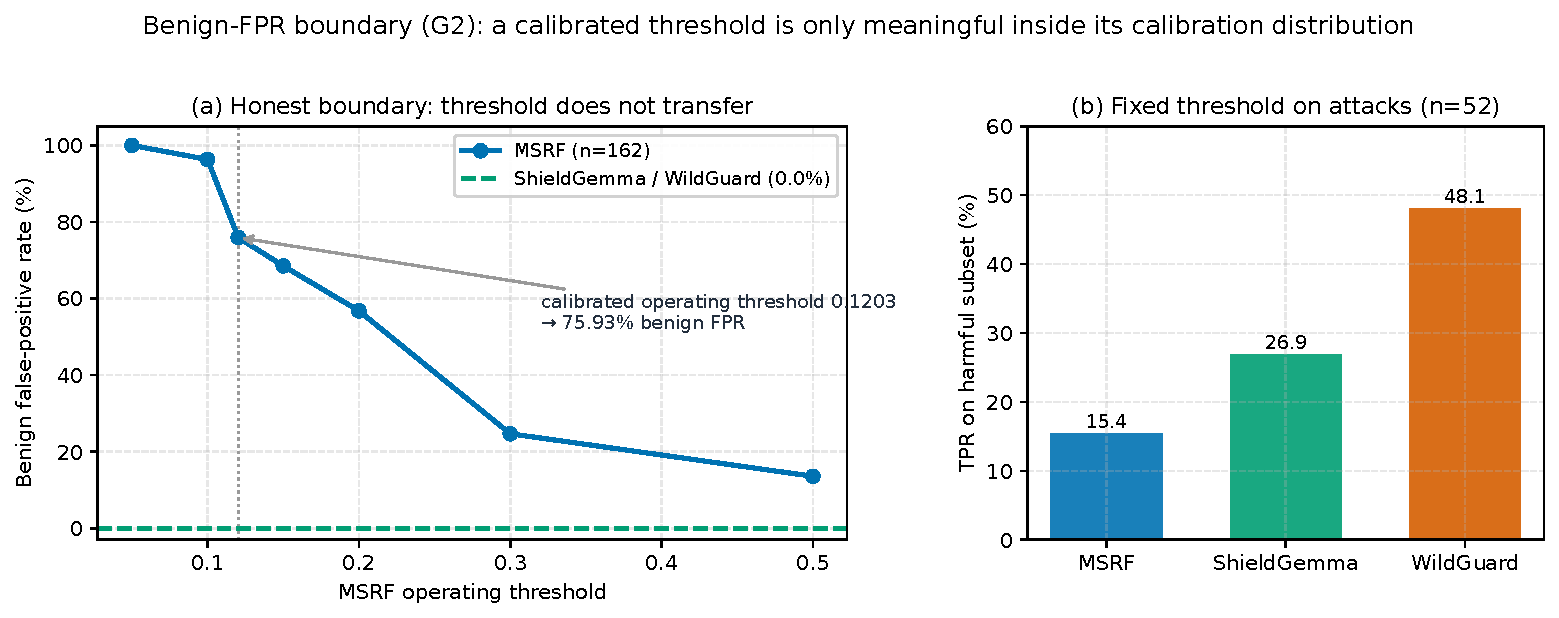
\includegraphics[width=0.88\textwidth]{figures/benign_fpr_boundary.pdf}
\caption{\textbf{Benign-FPR boundary (the G2 criterion).} Rendered as evidence
rather than avoided: (a) \MSRF{} false-positive rate on the independent benign
set ($n=162$) rises to \textbf{75.9\%} at the calibrated operating threshold
0.1203, versus 0.0\% for ShieldGemma and WildGuard; (b) at that \emph{fixed}
threshold, TPR on the harmful subset ($n=52$) is 15.4\% for \MSRF{}, 26.9\% for
ShieldGemma, and 48.1\% for WildGuard --- \MSRF's advantage is in-distribution
discrimination (AUC), not fixed-threshold hit rate on attacks.}
\label{fig:benign-fpr}
\end{figure}

% ======================================================================
% Robustness
% ======================================================================
\subsection{Robustness and adaptive attack}
\label{sec:robustness}

\subsubsection{Defense decay on the attack set}
On a separate attack set ($n=2{,}864$, gray-box and white-box perturbations, each
class $n\geq200$), we re-ran the guards at the response level. On the harmful
subset ($n=52$), \MSRF{} detects 15.4\%, ShieldGemma 26.9\%, WildGuard 48.1\%; on
all rows, \MSRF{} 19.1\%, ShieldGemma 11.3\%, WildGuard 22.2\%. We report these
numbers in full: \MSRF's advantage is in-distribution discrimination (AUC), not
fixed-threshold hit rate on attacks. We also disclose that the attack responses
carry no LoRA intent signal (the intent branch sees an out-of-distribution
zero), which explains part of the decay.

\subsubsection{Adaptive attack decay}
Against the real fused detector, gray-box and white-box perturbation classes
show detection-rate decay up to 20.0~pp relative to baseline. We scope the claim
precisely: our perturbations are single-pass, prompt-level transformations, not
iterative or gradient-based optimization, so we claim \emph{prompt-level
perturbation robustness}, not adversarial robustness in the gradient sense.
Three of six classes are effectively no-ops (fewer than half the perturbations
change the input) and are reported as such rather than as attacks.

\begin{figure}[t]
\centering
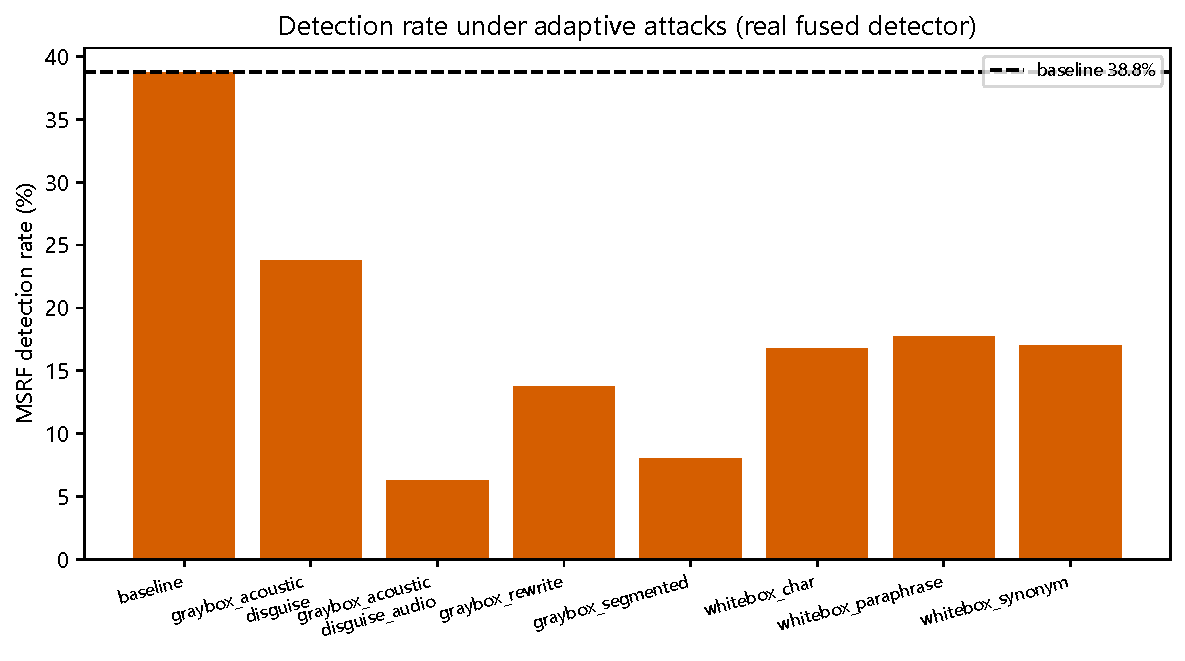
\includegraphics[width=0.72\textwidth]{figures/adaptive_decay.pdf}
\caption{\textbf{Detection-rate decay under adaptive perturbations.} The real
fused detector under gray-box and white-box adaptive perturbation classes,
with decay up to 20.0~pp relative to baseline. Perturbations are single-pass,
prompt-level transformations; we claim prompt-level perturbation robustness,
not gradient adversarial robustness.}
\label{fig:adaptive-decay}
\end{figure}

\subsubsection{Audio degradation}
Real audio degradation (Opus 16~kbps, SNR 20~dB, RIR reverberation, each EBU
R128-normalized) changes attack success in opposite directions across models
(e.g., $-7.0$~pp for E2B, $+11.3$~pp for E4B under Opus), which we report as-is.
Degraded audio increases ``thinking-trace leakage'' in one model
(10.0\% / 26.0\% / 28.5\% for the three degradations vs.\ 7.3\% baseline), and
that model's audio-side robustness must not be extrapolated to its text side,
where empty refusals reach 58--85\% (a genuine model behavior we report as such).

\subsubsection{Measurement trust chain}
\label{sec:trust-chain}
We report a five-layer trust chain: deterministic generation (byte-identical,
40/40); scorer reliability (judge\_big vs.\ judge\_small agreement 0.82 on
$n{=}3{,}573$ aligned cells, with Gwet's AC1 0.745 and balanced $\kappa$ 0.706
from the pipeline's agreement utilities \citep{cohen1968}); cross-family
scorer agreement (E4B side 0.929; full E2B text set 0.962); test--retest
agreement (1.000 across three scorers); and Dawid--Skene latent-label recovery
(0.945 in simulation at the measured error regime, 50 replications, 180 items,
$P(\mathrm{harm}){=}0.5$). Batch-inference
byte-equality is not guaranteed (42/200 cells byte-identical, zero errors),
which we disclose in the reproducibility statement.

\section{Discussion}
\label{sec:discussion}

\paragraph{Why narrative structure, and why does role assignment protect?}
The factorial results separate the ``storytelling'' bundle into a strong
structure effect (\Nfac{}) and a counter-intuitive protective effect (\Rfac{}).
A post-hoc account consistent with both is the elaboration-channel
hypothesis: \Nfac{}
increases elaboration (length, narrative density), which increases both the
probability and the perceived legitimacy of harmful continuations; \Rfac{}, by
contrast, constrains the model into an identity whose stance (an ``expert
advisor'') is at odds with producing harmful instructions in our protocol. The
replication of \Rfac's sign across models argues against a fluke, but its
sensitivity to the scoring caliber (it reverses under latent-label scoring)
demands caution; we report both.

\paragraph{Why do open-source guards fail on framing?}
ShieldGemma, WildGuard, and GradSafe all score below chance on framed inputs.
This is consistent with their training objective (harmfulness of direct
requests) being systematically mismatched with framing, which is
safe-looking. It motivates a \emph{knowledge} framing of the detection problem:
the relevant signal is not ``is this text harmful'' but ``does this structure
package harmful intent,'' which is exactly the signal our narrative and intent
branches measure.

\paragraph{Threshold detection versus mechanism-aware scoring.}
The benign-FPR failure (Section~\ref{sec:fusion-boundary}) is instructive rather
than incidental. It shows that a calibrated threshold is only meaningful inside the
calibration distribution, and that compliant benign behavior is statistically
confounded with framing signals. Read as a \emph{knowledge boundary} rather
than a defect, this is a substantive empirical finding about the framework's
applicability domain: the calibration pool (refusal responses) and the benign
pool (compliant responses) occupy different regions of the fused score space,
so the two distributions are not mutually calibrating. It is exactly this kind
of domain knowledge that our pre-registered defense gate G2 was designed to
elicit, and we report it in full. We argue that the honest contribution of a
fusion framework in this setting is a \emph{discriminative risk score with
auditable branch attributions} --- not a turnkey threshold --- and we present
the paper's detection claims accordingly. A direct path forward is
adaptive or online recalibration on deployment traffic, which we leave to
future work. This aligns with the journal's
orientation toward interpretable, decision-support knowledge systems
\citep{srd,realignment}.

\paragraph{Generalizability of the methodology.}
The contribution is best read as a \emph{methodology} rather than a tuned
detector. The four knowledge sources --- intent semantics, narrative structure,
acoustic prosody, and scoring uncertainty --- are defined from first principles
about the response and the scoring process, not about a specific model or
language; the causal protocol and the paired cross-modal measurement are
likewise model-agnostic. We therefore expect the framework to transfer to
other multimodal model audits (e.g., vision-language assistants whose safety
responses also admit packaging structure), to other high-resource languages,
and to high-stakes voice applications where an auditable, single-model risk
score is preferable to a stack of opaque classifiers. What transfers is the
\emph{structure}: mutually non-overlapping, auditable knowledge sources,
out-of-fold scoring, and honest boundary reporting. We have not re-run the
full protocol on these settings, and we state this explicitly rather than
claiming measured transfer.

\paragraph{Implications for knowledge-based decision systems.}
For the decision-support community, three design lessons follow. First, a
safety decision over a model response is a multi-source fusion problem. The
four signals we fuse are heterogeneous knowledge sources with different
reliability (the intent and narrative branches carry the signal; the acoustic
branch is ``not measured'', not ``ineffective''). Explicit calibration
plus an auditable fusion layer lets a system operator trace which source
drove a score. Second, the boundary between in-distribution discrimination and
threshold transfer is itself decision-relevant knowledge. The calibration pool
(adaptive refusals) and the benign pool (compliant responses) live in different
regions of the fused score space. A decision system must either keep its
operating context inside the calibrated region or re-calibrate online when the
deployment distribution drifts toward compliant benign traffic. Third, honest
boundary reporting is a decision-support feature, not a weakness: a score with
a documented failure region supports risk-informed routing (e.g., escalating
scores that fall outside the calibrated envelope to a human reviewer) better
than a threshold with an unmeasured false-positive rate. These are the
operational postures that follow from our measurement
\citep{guo2024survey,shafer1976,xu2025promethee}.

\section{Limitations}
\label{sec:limitations}

We report the principal limitations explicitly, each with the direction we
consider most promising for addressing it.
\begin{enumerate}[label=(\roman*)]
  \item \textbf{Scorer family bias.} All internal scorers are Gemma-family;
        cross-family anchoring bounds but does not eliminate this. Re-anchoring
        the protocol with at least one non-Gemma internal scorer to quantify
        the residual family bias directly is a natural next step.
  \item \textbf{Chinese-language scoring.} Only the dual-judge caliber is
        reliable on Chinese inputs; single-scorer Chinese results are not
        reported. Extending single-scorer Chinese reliability (e.g.,
        Chinese-native judges or scorer fine-tuning) is future work.
  \item \textbf{Acoustic factor confound.} \Asfac{} is implemented by voice,
        confounding speaker identity and gender; acoustic-attack signal is not
        measured at our sample window ($N=32$). Future work will separate
        voice identity from prosody (e.g., TTS with matched speaker identity)
        and enlarge the acoustic window well beyond $N=32$.
  \item \textbf{Length confound.} The effect is partially---not
        wholly---length-mediated; within matched length bands a content effect
        remains, and all three audio-channel estimators are reported.
        Additional matched-length designs and per-band estimators remain a
        planned extension.
  \item \textbf{Detection transfer.} Fixed-threshold detection fails on benign
        inputs (75.9\% FPR) and decays under adaptive attacks; only
        in-distribution discrimination and prompt-level robustness are claimed.
        Adaptive or online recalibration on deployment traffic, and an
        evaluation under gradient-based adversarial perturbations, are the
        natural next steps toward threshold transfer.
  \item \textbf{Out-of-distribution intent.} Attack responses lack the LoRA
        intent signal. Future work will add a LoRA intent signal at inference
        time or an explicit out-of-distribution guard on the intent branch.
  \item \textbf{Baseline coverage.} JailGuard, Cross-modal Information Check,
        and SALMONN-Guard were not reproducible (unreleased code/weights) and
        are reported as cited values only, never as measured baselines. We will
        re-run these baselines on release of their code or weights.
  \item \textbf{Sequential design.} The pre-registered maximum of 500
        cells\slash condition was exceeded by design change (v6.2$\rightarrow$v6.5),
        which we disclose. A cleaner confirmatory design within the original
        cap is future work.
  \item \textbf{Missing scorings.} 1.03\% of P0-C responses have deterministic
        parsing failures, bounded and disclosed. Re-scoring those cells with a
        robust parser is a planned cleanup.
\end{enumerate}

No fabricated values appear anywhere in this paper; every number traces to the
released pipeline artifacts.

\section{Conclusion}
\label{sec:conclusion}

We decomposed adversarial framing against large audio-language models into its
semantic components and showed, under an audited paired factorial protocol, that
narrative structure robustly increases attack success ($\Delta$27.9~pp, OR 16.65;
a larger agreement-conditioned dual-judge estimate is disclosed as inflated by
selection) across languages, models, and out-of-distribution inputs.
A substantial share of this effect is mediated by response elaboration, and
cross-modal safety divergence is model-dependent rather than modality-intrinsic.
We further introduced \MSRF{}, a 225-parameter knowledge-driven fusion framework
that discriminates framed attacks in-distribution (0.9784 ROC-AUC on the
deployment frame) while exposing its own boundary conditions honestly. Narrative
structure exhibits a robust causal effect under controlled prompt
interventions; representing that effect as structured, multi-signal knowledge
is, we argue, a more durable foundation for \LALM{} safety than either modal
shortcuts or opaque detection.

\section*{Data availability}
All pipeline artifacts, configurations, frozen seeds, and result files are
released in the anonymized companion repository accompanying this manuscript;
no pre-trained guard weights are redistributed.

\section*{Ethics}
All experiments use fabricated, synthetic harmful queries (never real personal
data), are confined to controlled research environments, and are reported under
a dual-use disclosure consistent with the study protocol and its gate decisions
(see the companion repository). The intent-classifier training data is
synthetic.

\section*{CRediT authorship contribution statement}
\textbf{Yongjin Chen}: Conceptualization, Methodology, Software, Validation,
Formal analysis, Investigation, Data curation, Writing -- original draft,
Writing -- review \& editing, Visualization.\\
\textbf{Songze Zhu}: Conceptualization, Methodology, Resources, Supervision,
Project administration, Funding acquisition, Writing -- review \& editing.

\section*{Declaration of competing interest}
None declared.

\section*{Funding}
This work was supported by the research project ``Data Black-Industry
Resilience: Generation Mechanisms and Governance Countermeasures''
(Grant No.\ 25CSH113).

\section*{Generative AI disclosure}
This manuscript was drafted with the assistance of AI writing tools for language
and organization; all experiments, measurements, and reported numbers are
human-executed and machine-verified.


\bibliographystyle{elsarticle-harv}
\bibliography{references}

\end{document}
